\chapter{Analysis method and efficiency correction}
\label{chap:methods}



\section{Selection and classification of events and tracks}
\label{sec:event_track_selection}
The selection criteria for validating events and tracks in a sample is of great importance since later measurements may be biased by these selections. The following describes which data sets were used and which conditions each event and each track had to meet in order to be considered in the further analysis. The entire analysis was developed in the \emph{ROOT} and \emph{AliROOT} frameworks which offer a high performance iteration through recorded events. 
 


\subsection{Event and track selection}
\label{sec:event_selection}
The analysis is performed on the \gls{pPb} collisions with a center-of-mass energy of $\sqrt{5.02}$\si{TeV} from the LHC13b and LHC13c periods with the second iteration of track reconstruction (pass2). For efficiency and closure investigations \gls{mc} generated events in period LHC13b2 (part 1-3, ``efix'')  were used. These events were generated by the Dual Parton Model based DPMJET event generator described in \cite{Roesler2000}. DPMJET implements the Reggeon theory for simulating soft, and perturbative \gls{qcd} for simulating hard events. \gls{mc} events which were not exposed to any simulated detector efficiencies are referred to as \gls{mc}-truth; and if they were, the are denoted as \gls{mc}-reconstructed.

Valid events are required to have a signal in both the V0A and V0C detectors\footnote{This corresponds to the AliRoot trigger bit AliVEvent::kINT7}. Furthermore, the events' reconstructed vertex position are required to be within $\pm \SI{10}{cm}$ of the detector's center along the beam axis (\zvtx).

This analysis focuses on tracks which are primary particles reconstructed in the ITS and TPC\footnote{The exact filter used was filter bit $10$ corresponding to\newline AliESDtrackCuts::GetStandardITSTPCTrackCuts2011(kTrue, 0)}. These tracks are commonly referred to as \gls{golden} tracks. In order to investigate the sensitivity of the analysis to the choice of track cuts, the so called \gls{TPC-only}\footnote{This corresponds to filter bit $10$ or  AliESDtrackCuts:GetStandardTPCOnlyTrackCuts()} cuts were also used in some instances. The difference between the tracks are that the golden tracks requires associated hits in the \gls{spd} and are therefore less likely to include secondary tracks from e.g. weak decays of heavy quarks, but they have lower efficiency and an asymmetric $\varphi$ acceptance due to \gls{spd} cooling issues that meant that not all sectors could be operated. \gls{TPC-only} tracks are required to have a  \gls{dca} to the reconstructed interaction vertex of less than \SI{2.4}{cm} transverse and \SI{3.2}{cm} parallel to the beam direction while golden tracks have a \pt dependent \gls{dca} cut that is in general much tighter.

\subsection{Enriching the sample with hard events}
\label{sec:enrich_hard}

In order to investigate the dependence of any observable on the hardness of the underlying interaction an additional event selection criterion was introduced.
The definition of a hard event is similar to the one given in \cite{Acosta2002} and assumes that a hard parton interaction develops into a high \pt final particle.
The enriched hard sub sample is then produced by requiring at least one valid track with a \pt value above a given threshold \ptthresh. 

\subsection{Multiplicity classes}
\label{sec:mult_classes}
Picturing the \gls{Pb} nucleus as an extended object it is possible to define centrality as a parameter of the collision geometry. The centrality estimation used for this analysis is outlined in \cite{Morsch2013,ALICECollaboration2012}. 

The more central a collision is the more binary collisions $N_{coll}$ will occur, i.e.\ the centrality is given by an estimator depending monotonically on the number of collisions. Subsequently, $N_{coll}$ is connected to the number of measurable charged particles via the Glauber model. Thus the centrality of a collision may be estimated by measuring its number of charged tracks $N_{ch}$. However, a lot of work has been ongoing in ALICE to link multiplicity to centrality but this is not yet quantitatively well understood for \gls{pPb} collisions. The problem arises from the relatively large fluctuations (in comparison to \gls{PbPb}) in $N_{ch}$ for a fixed value of $N_{coll}$ causing different detectors to have different biases \cite{Morsch2013}.Thus throughout the following, the more general term ``multiplicity'' will be used instead of the debated and more model-dependent ``centrality''. Nevertheless, the two terms describe essentially the same property of an event.\\

As presented in sec. \ref{sec:detectors}, \gls{alice} has a number of detectors capable of measuring multiplicities covering various pseudo rapidity ranges. Commonly the total charged deposited in either one or both of the V0 detectors is used to deduce the multiplicity of the underlying event. If the sum of  V0A and V0C is used in the multiplicity determination the method is referred to as \emph{V0M}; if only the counts yielded by VZEROA are processed the estimator is also called \emph{V0A}. The latter one was used in this analysis.


In order to study the multiplicity dependence of two particle correlations four event classes were defined as ranges in the measured multiplicity. The classes are labeled according to the sections in the distribution of the number of events detected with each such multiplicity. This distribution is depicted in fig.~\ref{fig:V0A_dist}. Hence, the classes are labeled as $(0-20\%)$, $(20-40\%)$, $(40-60)\%$ and $60-100\%$; the first exhibiting the highest, the last the lowest multiplicity. 

\begin{figure}
  \centering
  \includegraphics[width=.8\textwidth]{figures/cent_V0A.pdf}
  \caption[Distribution of the total deposited charge in the VZEROA detector per event.]{Distribution of the total deposited charge in the VZEROA detector per event. Multiplicity classes are defined as percentile of this distribution. Simulated data from the Glauber model is shown in red. From \cite{V0Acent2013}}
  \label{fig:V0A_dist}
\end{figure}

\section{The correlation function}
\label{sec:correlation_function}

Two-particle correlation functions are a popular tool to investigate the structure and properties of the created medium in heavy ion physics. These correlations reflect direct correlations due to e.g.\ particles originating from the same jet, but may also contain indirect correlations like the flow correlations in heavy ion collisions where particles are correlated through the event planes. The aim of the here presented method is to remove the direct hard component in order to facilitate further studies of the double-ridge structure described in sec. \ref{sec:flow-like-pPb} that can shed light on its unknown origin.


In the following analysis, the two-particle correlations are not calculated for all tracks produced by an event. Instead two \pt intervals, namely a \emph{trigger} and an \emph{associated} interval, are defined. The transverse momentum of a particle of the former interval is denoted by \pttrig while the latter one is referred to as \ptassoc. Correlations are extracted from an event by calculating the azimuthal ($\Delta\varphi$) and pseudo rapidity ($\Delta \eta$) differences between each trigger and the associated particles.

\subsection{Signal distribution}
\label{sec:signal_distribution}
The correlation function $S(\Delta\eta, \Delta\varphi)$, from here on denoted as \emph{signal distribution}, for an ensemble of $N_{\text{events}}$ events is then defined as
\begin{equation}
  \label{eq:signal}
  S(\Delta\eta, \Delta\varphi) = \frac{1}{\sum_{N_{\text{events}}} N_{\text{trig}}}
  \sum_{N_{\text{events}}} 
  \sum_{N_{\text{trig}}}
  \frac{d^2N_{asso}^{same}}{d\deta d\dphi}
\end{equation}
where $N_\text{trig}$ ($N_{asso}^{same}$) denote the number of triggers (associated) particles per event. Computing $\Sig$ from experimental data will not, however, yield a correlation distribution similar to the one shown in fig. \ref{fig:double_ridge_pPb} (left). Instead it will appear in a triangular shape along \deta as is shown in fig. \ref{fig:example_signal}. The origin of this distortion lies in the finite acceptance within the limits $\pm\eta_m$ of the detector. A trigger found at $\eta = 0$ may contribute to the signal distribution within the \deta interval $\left[-\eta_m, \eta_m\right]$, while a trigger found at $\eta = -\eta_m$ may only contribute within the range of $\left[-2\eta_m, 0\right]$. Thus, any trigger may contribute to the signal at $\deta = 0$ but the number of triggers contributing to non central regions of $\Sig$ decreases linearly\footnote{In fact it is not quit lineary as discussed in the following section} with \deta yielding the triangular shape of $\Sig$. It is important to emphasize that a perfect detector with infinite acceptance in $\eta$  would indeed yield a \Sig similar to the ones shown in fig. \ref{fig:double_ridge_pPb} (left). Furthermore,  no such acceptance-based distortions are expected along \dphi due to the full azimuthal acceptance of the detector in practice.

The next two sections discuss the correction of this distortion  which is necessary to isolate the underlying genuine correlations.

% Peters comment:
% Maybe add somewhere:
% We expect that there is a direct correlation due to the trigger and associated being related to the same hard back-to-back process but wants primarily here to look for the underlying not understood association implied by the double ridge.

%\subsection{Signal distribution}
%\label{sec:signal_distribution}
% \begin{figure}[htbp]
%   \centering
%   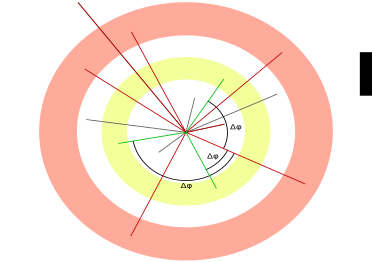
\includegraphics{figures/trigger_assoc.pdf}
%   \caption{Schematic concept for the introduction of \pt intervals for the two particle correlation depicting a collision and its tracks along the beam axis. The length of a track represents its \pt value, the polar angle represents $\varphi$. The light red (green) zone represents the trigger (associated) interval. Tracks falling into each category are marked appropriately. Angular differences are shown as an example for one trigger.}
%   \label{fig:trigger_assoc}
% \end{figure}

% Applying eq. (\ref{eq:correlation}) to experimental data will not, however, yield correlation distributions similar to those depicted in fig. \ref{fig:double_ridge_pPb} (left hand side). Instead 
% If one drops the assumption of no genuine correlation made for $B$ one has to anticipate not only additional structure along \deta but also along $\dphi$;  some azimuthal differences between trigger and associated particles will be more likely than others. Such a distribution is referred to as signal distribution $S(\deta, \dphi )$ in the following. Its formulation is naturally very similar to eq. (\ref{eq:background_datadriven}) but weighted to the total number of triggers in the given multiplicity class and \zvtx section in the detector:
% \begin{equation}
%   \label{eq:signal}
%   S(\deta, \dphi) = \frac{1}{N_{trig}}
%   \sum_{N_{\text{events}}} 
%   \sum_{N_{\text{trig}}}
%   \frac{d^2N_{asso}^{same}}{d\deta d\dphi}
% \end{equation}
% where $N_{asso}^{same}$ denotes the number of associated particles of a given event. An example for $S(\deta, \dphi)$ is depicted in fig. \ref{fig:example_signal}.


\begin{figure}[htbp]
  \centering
  \begin{subfigure}[b]{0.5\textwidth}
    \includegraphics[width=\textwidth]{figures/example_signal.pdf}
    \caption{Signal distribution example}
    \label{fig:example_signal}
  \end{subfigure}%
  \begin{subfigure}[b]{0.5\textwidth}
    \includegraphics[width=\textwidth]{figures/example_background.pdf}
    \caption{Background distribution example}
    \label{fig:example_backgroun}
  \end{subfigure}
  \caption[Examples of signal and background distributions from experimental data.]{Examples of signal and background distributions from experimental data in the trigger (associated) interval of $1 < \ptassoc < \SI{2}{GeV/c}$ ($2 < \pttrig < \SI{4}{GeV/c}$) for golden track cuts. The distributions appear distorted along \deta mainly due to small differences in pseudo rapidity being accessible to a greater amount of trigger-associated pairs than large \deta values.}
  \label{fig:example_signal_background}
\end{figure}


\subsection{Background distribution}
\label{sec:background_distribution}
The acceptance is indeed the main contribution to the discussed distortions (referred to as \emph{Background} \B in the following) but not the sole. In order to correct \Sig for any non physics related distortions it is crucial to understand their origins. A analytical description of \B, which is in fact an \emph{autocorrelation} function, will be presented first. Subsequently, the data-driven approach for extracting \B which was applied in the latter studies will be introduced. 

The following focuses on the \deta variable but all arguments are also applicable to the \dphi coordinate. Firstly, it is helpful to analytically define the former mentioned detector acceptance as:
\begin{equation}
  \label{eq:acc}
  a(\eta ) =
  \begin{cases}
  1 & \text{if } |\eta| < \eta_m \\
  0 & \text{everywhere else}
  \end{cases}
\end{equation}
i.e.\ particles within the cuts are included all particles outside the cuts are excluded.

The next source of autocorrelations to be discussed stems from the detector efficiency $\epsilon$ which in general dependents on $\eta$ (see sec. \ref{sec:single-track-corr} for a thorough discussion of $\epsilon$). Its effect on the two-particle correlation function may be illustrated as follows. If two regions of the detector were to exhibit a higher efficiency than all other regions it is easy to picture that the $S(\deta)$ will show an enhancement at $\deta = 0$ and for the angular distance \deta between these two regions. 

Lastly, the same argument as for the efficiency may also be applied to the particle density $dN/d\eta$. Two regions with a high particle densities would again yield an increased correlation at $\deta = 0$ and at the angular distance between the two regions.\\

Having identified these three sources for the distortion of \Sig one can now define $B(\eta)$ in the following way \cite{Xu2013, Schuster2013}:
\begin{align}
  \label{eq:fancy_bg_1}
  B(\Delta\eta) &\propto \int_{-2\eta_m}^{2\eta_m} d\eta f(\eta) f(\eta - \Delta\eta) \\
  \label{eq:fancy_bg_2}
  f(\eta) &= a(\eta) \cdot \epsilon(\eta) \cdot \frac{dN(\eta)}{d\eta}
\end{align}
Assuming that $\epsilon(\eta)$ and $dN/d\eta$ are constant eq.~(\ref{eq:fancy_bg_1}) would yield the simplified picture of a triangular shape described in sec. \ref{sec:signal_distribution}. As stated initially, the same arguments hold for the \dphi variable the only difference being that the acceptance and particle density are constant within the integration region. An example of a \B as it was used in the latter analysis is shown in fig.~\ref{fig:example_backgroun}.\\

\B could now be constructed from the measured particle density $dN/d\eta$, the known detector acceptance and an efficiency derived from \gls{mc} detector simulations. This approach is very complex and error prone and an alternative way of retrieving \B purely from measured data exists. It is based on the idea that $\Sig \propto \B$ if \Sig is constructed from associated tracks which are entirely uncorrelated to the trigger particle. This can be achieved by pairing an event's trigger particles to associated ones from many other, independent events. However, close care has to be taken that all tracks involved in this \emph{event mixing} have a similar efficiencies $\epsilon$ and particle distributions $\frac{dN}{d\eta}$. This is ensured by choosing associated particles from events within the same \zvtx interval and multiplicity class as the event of the trigger particle.
Hence, a data-driven background distribution for $N_{events}$ within a given multiplicity class and \zvtx section can thus be expressed as
\begin{equation}
  \label{eq:background_datadriven}
  B(\deta, \dphi) = \alpha \alpha_{corr}
  \sum_{N_{\text{events}}} 
  \sum_{N_{\text{trig}}}
  \frac{d^2N_{asso}^{mixed}}{d\deta d\dphi}
\end{equation}
where $\alpha$ is a constant normalizing the background to unity for points with maximal two-particle acceptance, i.e.\  $B(\deta = 0, \dphi=0) \approx 1$. $\alpha_{corr}$ is a correction to this normalization described below.

$N_{asso}^{mixed}$ denotes the number of associated tracks with no genuine correlation to the trigger particle. In practice, these associated particles are chosen from a \emph{pool} of formerly processed events which have the \zvtx within $\pm \SI{2}{cm}$ of the trigger's event vertex and are of the same multiplicity class. Since the \B is a normalized distribution it is possible to decrease statistical uncertainties by increasing the number of uncorrelated associated particles. In this analysis each processed event was mixed with ten times the number of its associated tracks. Once the event mixing was completed for a given event, a random set of tracks in the pool was replaced by the associated particles of the current event.

When performing the afore mentioned normalization of  $B(\deta, \dphi)$ it is important to take into account the finite bin width of the histogram; i.e.\ the most central bins of $B(\deta)$ have to be below unity as is depicted in fig. \ref{fig:norm_bg}. This is achieved by the correction $\alpha_{corr}$. Since the analytic shape of \B is not know it is approximated by the acceptance triangle given as $B(\deta) / \alpha \approx 1-1.0/\eta_m|\deta|$. Thus, $\alpha_{corr}$ is given by
\begin{equation}
  \label{eq:alpha}
  \alpha_{corr} = 1- \frac{\deta^{\text{width}}}{\eta_m}
\end{equation}
where $\deta^{\text{width}}$ is the \deta bin width used in the analysis.

\begin{figure}
  \centering
  \includegraphics[]{figures/finite_binwidth_correction.pdf}
  \caption{Example of the finite bin width correction as applied to the normalization of  the background distribution \B.}
  \label{fig:norm_bg}
\end{figure}

\subsection{Total associated yield}
\label{sec:total_yield}
As stated above, any genuine correlation will cause a deviation between the Signal distribution $S(\deta, \dphi)$ and the background distribution $B(\deta, \dphi)$. However, it is a topic of current research \cite{Schuster2013} how the physical  correlations combine with the background to yield the measured signal. This analysis follows the standard \gls{alice} procedure described below and discusses the arguments brought forth in appendix \ref{sec:in_depth_Y}.

The signal corrected for the background is referred to as \emph{total associated yield per trigger particle}\footnote{Distribution of associated particles with respect to a trigger particle} and denoted as $Y(\deta, \dphi)$. \Y is in this analysis defined within a given multiplicity class and \zvtx interval as
\begin{equation}
  \label{eq:total_yield}
  Y^{\zvtx}(\deta, \dphi) \approx
  \frac{1}{N^{\zvtx}_{trig}}\frac{d^2N_{assoc}}{d\deta d\dphi} =
  \frac{S(\deta, \dphi)}{B(\deta, \dphi)}
\end{equation}
This definition ensures that \Y is flat if no correlations between the trigger and associated particles are present. Fig. \ref{fig:example_y} depicts \Y for the signal and background distribution shown in fig. \ref{fig:example_signal_background} revealing the common di-jet structure of \gls{pPb} events.

Finally, all \zvtx intervals may be combined by a summation weighted by the number of triggers in each interval.

\begin{figure}
  \centering
  \includegraphics[width=0.5\textwidth]{figures/example_y.pdf}
  \caption[Total associated yield \Y retrieved from the distributions shown in fig. \ref{fig:example_signal_background} using the definition of eq. (\ref{eq:total_yield}).]{Total associated yield \Y retrieved from the distributions shown in fig. \ref{fig:example_signal_background} using the definition of eq. (\ref{eq:total_yield}). The di-jet structure common to \gls{pPb} collisions is clearly visible.}
  \label{fig:example_y}
\end{figure}

\section{Visual repesentation of two dimensional histograms}
\label{sec:multi_plot_expl}
During the course of this project it was found that the visual representation of two dimensional histograms as depicted in fig. \ref{fig:example_y} may be deceiving. They do not allow for precise quantitative comparison and often it is more illuminating to examine the projections onto the \deta or \dphi axis. Thus, it was decided to replace the three dimensional representation seen in fig. \ref{fig:example_y} with a two dimensional ``heat map'' where ``hot'' (red) are high values and ``cold'' (blue) are low values. This has the advantage of not depending on a viewing angle while still granting a good overview of the histogram. Furthermore, this heat map shares its \deta and \dphi axes with projection performed onto each respective axis.

Several examples of such a combined plot, which will be used extensively in the following, may be seen in fig.~\ref{fig:effect_single_track_correction}. In the shown cases the \dphi projection (top) was performed and averaged over the entire \deta range. Chapter \ref{chap:results} will include instances where the \emph{peak region} $(|\deta|< 0.8; |\dphi| < \pi /2)$ was excluded from this projection. The right hand part of the combined plot shows projections onto \deta for different regions of the histogram: The \gls{near-side} ($|\dphi| < \pi /2$), \gls{away-side} ($\pi /2 < \dphi < 3\pi/2$) and remaining regions\footnote{These definitions are used throughout the reminder of this thesis.}.  This differentiation helps to identify and quantitatively compare \dphi dependent structures in the two dimensional projection (e.g.\ correlations in $S(\deta, \dphi )$ as described in sec. \ref{sec:signal_distribution}).


\section{Efficiency correction}
\label{sec:effic-corr}

\subsection{Pair-efficiency correction}
\label{sec:single-track-corr}
Depending on the cuts chosen for a given analysis, the probability of a given particle being successfully reconstructed depends on its $\eta$, $\varphi$, \pt and \zvtx. An efficiency function $\epsilon(\eta, \varphi, \pt, \zvtx)$ can be computed from the simulated reconstruction of MC-truth events in the detector. The efficiency is then given by
\begin{equation}
  \label{eq:eff_theo}
  \epsilon (\eta, \varphi, \pt, \zvtx) =
  \frac{d^4N_{\text{mc-recon}}}{d\eta d\varphi d\pt d\zvtx} /
  \frac{d^4N_{\text{mc-truth}}}{d\eta d\varphi d\pt d\zvtx}
\end{equation}
where $N$ is the total number of particles in the given collection of events. The correction is then applied by weighting each associated-trigger pair in \Sig and \B by $1/(\epsilon^{\text{trig}}\epsilon^{\text{assoc}})$ where $\epsilon^{\text{trig}}$ is the efficiency for the trigger particle and $\epsilon^{\text{assoc}}$ for the associated one. This method is referred to as \emph{pair efficiency correction} in the following and represents the correction method applied in the majority of all correlation studies\cite{Schuster2013,Abelev2012}. However, the following section shows that it is possible to exploit the definition of the total associated yield per trigger particle given in eq.~(\ref{eq:total_yield}) in a way that replaces the entire efficiency correction procedure described above by a simple scaling of the final distribution. 


\subsection{Correction by average detector efficiency in \ptassoc interval}
\label{sec:single-value-correction}

A common principle in experimental particle physics is to strive for an analysis which is as model independent as possible and does not include layers of complexity which do not improve the yielded results. In this spirit a new approach for treating detector efficiencies was developed and deployed during this thesis. 

The starting point is eq.~(\ref{eq:total_yield}) which defined in this way in order to correct the autocorrelations represented by \B in \Sig. Equation (\ref{eq:fancy_bg_2}) shows that the autocorrelations stem from (generalizing to two dimensions) $\frac{d^2dN}{d\eta d\varphi}$, the detector acceptance  $a(\eta, \varphi)$ and $\epsilon(\eta, \varphi)$. Assuming that the event mixing was flawless, all three of these are identical for \Sig and \B. This means that by taking the ratio of these two quantities one corrects for all the autocorrelations caused by $\frac{d^2dN}{d\eta d\varphi}$,  $a(\eta, \varphi)$ and $\epsilon(\eta, \varphi)$. Hence, the question arises what one gains by correcting the effects of the detector efficiencies individually in \Sig and \B as described in sec. \ref{sec:single-track-corr} if the definition of \Y would correct for the autocorrelations caused by $\epsilon(\eta, \varphi)$ anyways? This may be illustrated by computing  $Y^{uncorr}$ from uncorrected MC reconstructed data and  $ Y^{pair-corr}$ from corrected MC reconstructed data. Fig. \ref{fig:effect_single_track_correction} shows the ratio $Y^{uncorr}/Y^{pair-corr}$ for the intervals $0.5 < \ptassoc < \SI{1}{GeV/c}$ and $1 < \pttrig < \SI{2}{GeV/c}$.

\begin{figure}
  \centering
  \includegraphics[]{figures/single_track_corr_effect.pdf}
  \caption[Ratio of two total associated yields per trigger particles, one computed without efficiency corrections applied, the other being corrected by a  pair-efficiency correction.]{Ratio of two total associated yields per trigger particles, one computed without efficiency corrections applied, the other being corrected by a  pair-efficiency correction. The obtained distribution is flat along \deta and \dphi. The baseline of the distribution coinciedes well with the average detector efficiency in the given \ptassoc interval of $0.5 < \ptassoc < \SI{1}{GeV/c}.$}
  \label{fig:effect_single_track_correction}
\end{figure}

As anticipated from the above discussion, no deviation from a flat distribution outside the statistical uncertainties is present. However, $Y^{uncorr}$ is scaled by the factor $\sim 0.807$ in comparison to $Y^{pair-corr}$. This factor coincides with the detector efficiency averaged over the acceptance region and \ptassoc interval to approximately $\pm 0.5\%$ in all studied intervals of \ptassoc and $\pttrig$ and even when applying the high \pt threshold. Furthermore, some quantities, like e.g.\ the $v_2$ are not even sensible to the error in the scaling. The ridge yields described in sec. \ref{sec:yield_extraction}, on the other hand, are sensible but are limited by other statistical systematic uncertainties.\\

Thus, this correction method, in the following referred to as \emph{average efficiency method}, proofed sufficiently precise and easier to apply than the pair-correction method while also exposing the inherent independence of the two-particle correlation function onto the precise topology of the efficiency distribution and the track cuts chosen. Therefore, all of the following results were corrected by this method unless otherwise noted.


\section{MC closure test}
\label{sec:mc-closure}
A closure test probes if a given correction method applied to reconstructed data yields the original MC truth results. In the case of this analysis $B$, $S$ and $Y$ were computed for the MC truth as well as for the reconstructed data. In case of the latter, the pair-efficiency correction as described in section \ref{sec:single-track-corr} was applied to the associated tracks since a correction of \Sig an \B with the average efficiency method is not possible. The closure test was then performed by dividing the distributions retrieved from the reconstructed data by those based on the MC truth events.

\subsection[MC closure test without high \pt threshold]{MC closure test without high \ptbold threshold}
\label{sec:closure_no_thresh}
Results of the MC closure test for \Sig and \B at $0.5 \le \ptassoc \le \SI{1}{GeV/c}$ and $1 \le \pttrig \le \SI{2}{GeV/c}$ are depicted in fig. \ref{fig:closures}. Since the average-efficiency correction is only applicable to \Y the left hand plots were generated from uncorrected reconstructed data while the right hand ones were corrected by pair-efficiency correction as described in sec. \ref{sec:single-track-corr}. The most peripheral event class ($60-100\%$) was chosen as an example since it demonstrates the strongest deviations from the MC truth. The ratio below one in the former was to be expected since the number of reconstructed associated particles per event is always less or equal to the their count in MC truth. The pair-efficiency correction is found not to lead to MC closure for $S$ and $B$ while introducing additional structure along \deta.
\begin{figure}
  \centering
  \begin{subfigure}[b]{0.5\textwidth}
    \includegraphics[width=\textwidth]{figures/closure_S_peri_no_st.pdf}
  \end{subfigure}%
  \begin{subfigure}[b]{0.5\textwidth}
    \includegraphics[width=\textwidth]{figures/closure_S_peri_st.pdf}
  \end{subfigure}
  \begin{subfigure}[b]{0.5\textwidth}
    \includegraphics[width=\textwidth]{figures/closure_B_peri_no_st.pdf}
  \end{subfigure}%
  \begin{subfigure}[b]{0.5\textwidth}
    \includegraphics[width=\textwidth]{figures/closure_B_peri_st.pdf}
  \end{subfigure}
  \caption[Ratios between results from reconstructed and MC truth analysis for peripheral events ($60-40\%$) at the detector center.]{Ratios between results from reconstructed and MC truth analysis for peripheral events ($60-40\%$) at the detector center. The trigger and associated intervals are chose as $0.5 \le \ptassoc \le \SI{1}{GeV/c}$ and $1 \le \pttrig \le \SI{2}{GeV/c}$. Plots on the left hand side show uncorrected results. The reconstructed data for the plots on the right hand side was corrected by pair-efficiency correction as described in sec. \ref{sec:single-track-corr} thus representing a MC closure test. The top row shows the ratios for $S$, the bottom row for $B$. Pair-efficiency correction does not lead to closure for $S$ and $B$ and introduces additional structure in \dphi when compared to the uncorrected ratios.}
  \label{fig:closures}
\end{figure}

However, when calculating $Y(\deta, \dphi)$, which was left uncorrected (left) for the sake of comparison to fig.~\ref{fig:closures},  these structures were found to cancel each other. As depicted in fig. \ref{fig:closure_Y} both, the uncorrected as well as pair-efficiency corrected \Y showed minimal structure along \deta and \dphi. Furthermore, the pair-efficiency corrected MC closure test yielded a baseline just $\sim 0.5\%$ above unity; i.e.\ the pair-efficiency correction reproduced the MC data to a good approximation.

\begin{figure}[htbp]
  \centering
  \begin{subfigure}[b]{0.5\textwidth}
    \includegraphics[width=\textwidth]{figures/closure_Y_peri_no_st.pdf}
  \end{subfigure}%
  \begin{subfigure}[b]{0.5\textwidth}
    \includegraphics[width=\textwidth]{figures/closure_Y_peri_st.pdf}
  \end{subfigure}
  \caption[Ratios between the total associated yield $Y$ computed from reconstructed and MC data for peripheral events ($60-40\%$).]{Ratios between the total associated yield $Y$ computed from reconstructed and MC data for peripheral events ($60-40\%$). The trigger and associated intervals were set as $0.5 \le \ptassoc \le \SI{1}{GeV/c}$ and $1 \le \pttrig \le \SI{2}{GeV/c}$. The left hand plot shows the uncorrected result. The reconstructed data of the plots on the right hand side was corrected by pair-efficiency correction as described in sec. \ref{sec:single-track-corr}. The \dphi structures observed in \ref{fig:closures} appears to cancel when calculating $Y$ for both corrected and uncorrected results. ``Closure'' may be achieved for the uncorrected data by scaling $Y$ by a constant value.}
  \label{fig:closure_Y}
\end{figure}

However, non-closure was observed for other intervals of \ptassoc and \pttrig than the one described above. Fig. \ref{fig:non-closure_2-4_no_thresh} displays the ratio of \Yrecon and \Ytruth for the  $0-20\%$ (left) and $60-100\%$ (right) multiplicity classes. A di-jet-like structure emerged in the latter case whose origin is currently not yet understood. The non closure becomes more severe when applying a high \pt threshold.

\begin{figure}
  \centering
  \begin{subfigure}[b]{.5\textwidth}
    \includegraphics{figures/no-closure-uncorrected-cent.pdf}    
  \end{subfigure}%
  \begin{subfigure}[b]{.5\textwidth}
    \includegraphics{figures/no-closure-uncorrected.pdf}    
  \end{subfigure}
  \caption[MC closure test pass for the ($0-20\%$) and ($60-100\%$) multiplicity class.]{MC closure test pass for the ($0-20\%$) class (left) and fails for ($60-100\%$) in the associated and trigger intervals of $0.5 \le \ptassoc \le \SI{1}{GeV/c}$, $2 \le \pttrig \le \SI{4}{GeV/c}$. The origin of this non closure is not yet understood.}
  \label{fig:non-closure_2-4_no_thresh}
\end{figure}

\subsection{Non closure due to event mixing}
\label{sec:sensitivity_pool_composition}

It should be noted that the entire analysis is very sensitive to the composition of the event mixing pool. Figure \ref{fig:wrong_pool} shows the effects of a pool including events which do not have any trigger but are otherwise valid. Those events do not contribute to $S$ but appear to have different particle densities $dN/d\eta$ than events with one or more triggers. Hence, following the argumentation in section \ref{sec:total_yield}, the resulting total yield appears distorted along \deta. Some other ALICE correlation analysis \cite{Schuster2013} have had similar problems with so called \emph{wings} in \deta which might very well be related to such biases introduced with the event mixing.

\begin{figure}
  \centering
  \includegraphics{figures/closure_bad_pool_example.pdf}
  \caption[Effect of an event pool not precisely reflecting the event selection criteria of events in the signal distribution $S$.]{Effect of an event pool not precisely reflecting the event selection criteria of events in the signal distribution $S$. Events having no trigger were used in the event mixing while they were not contributing to $S$.}
  \label{fig:wrong_pool}
\end{figure}


\subsection[MC closure with high \pt threshold]{MC closure with high \ptbold threshold}
\label{sec:closure_with_thresh}

Applying the high \pt threshold \ptthresh as described in sec.~\ref{sec:enrich_hard} and hence dividing the event sample into \gls{soft} and \gls{hard} poses further complications regarding the MC closure test for the analysis method at hand. Again, it should be noted that it is crucial that the events used in the event mixing are as similar as possible to the ones use in the calculation of $S$. It was found that not applying the threshold criteria to the mixing events leads to a distortion along \deta analog to the one described above and depicted in fig. \ref{fig:wrong_pool}. 

Albeit, even if \ptthresh is properly applied in the event mixing, MC-closure was not achieved for all event classes simultaneously in any tested \ptassoc and \pttrig interval. Instead, a di-jet structure, similar to the one discussed in sec.~\ref{sec:closure_no_thresh}, emerged for decreasing multiplicity as is shown in fig. \ref{fig:closure_structure_w_threshold}.
\begin{figure}
  \centering
  \begin{subfigure}[b]{0.5\textwidth}
    \includegraphics[width=\textwidth]{figures/closure_structure_class_0.pdf}
  \end{subfigure}%
  \begin{subfigure}[b]{0.5\textwidth}
    \includegraphics[width=\textwidth]{figures/closure_structure_class_1.pdf}
  \end{subfigure}
  \begin{subfigure}[b]{0.5\textwidth}
    \includegraphics[width=\textwidth]{figures/closure_structure_class_2.pdf}
  \end{subfigure}%
  \begin{subfigure}[b]{0.5\textwidth}
    \includegraphics[width=\textwidth]{figures/closure_structure_class_3.pdf}
  \end{subfigure}
  \caption[MC closure tests for all four multiplicity classes.]{MC closure tests for all four multiplicity classes with the associated and trigger intervals at $0.5 \le \ptassoc \le \SI{1}{GeV/c}$, $2 \le \pttrig \le \SI{4}{GeV/c}$ and a threshold of \SI{4}{GeV/c}. A di-jet like structure emerges with decreasing multiplicity.}
  \label{fig:closure_structure_w_threshold}
\end{figure}

The following attempts were made to understand the origin of the non closure:

\begin{itemize}
 \item The computations were repeated for the \gls{TPC-only} event cuts (\gls{golden} track cuts were used in fig. \ref{fig:closure_structure_w_threshold}). As described in section \ref{sec:event_selection}, the former cuts are flat along $\varphi$ while the latter ones exhibit significant gaps. The result for the most peripheral event class, exhibiting the most significant structure, is displayed in fig. \ref{fig:investigate_non_closure} (left hand side). Evidently, the same \gls{di-jet} like structure emerged in the \gls{TPC-only} cut as was observed in \gls{golden} cuts. This observation is also in agreement to the considerations made when defining the average-efficiency correction in sec.~\ref{sec:single-value-correction}. Hence, it can be excluded that the observed non closure originates from detector deficiencies.
 \item Appendix \ref{sec:st_shortcomings} describes a bias towards events with many triggers, due to detector deficiencies and the definition of the two-particle correlation function. The effect of this bias was investigated by only considering events which have exactly one generated trigger particle at the generator level. Thus, any possible bias towards events with many triggers was eliminated. Enforcing that new requirement yielded the $\Yrecon / \Ytruth$ ratio shown in fig. \ref{fig:investigate_non_closure} (right hand side). Neither the \deta nor the \dphi structures were significantly altered by the described limitation of the sample. Thus, the non closure seems to not stem from a event selection depending on the number of MC truth triggers in an event. 
\end{itemize}

\begin{figure}[htbp]
  \centering
  \begin{subfigure}{0.5\textwidth}
    \includegraphics[]{figures/closure_TPC.pdf}
  \end{subfigure}%
  \begin{subfigure}{0.5\textwidth}
    \includegraphics[]{figures/closure_TPC_one_mc_trigger.pdf}
  \end{subfigure}
  \caption[Investigation into the origin of non closure by changing changing event selection criterion and track cuts.]{Investigation into the origin of non closure. Depicted are the cases for most peripheral events using TPC-only cuts in the associated and trigger intervals of $0.5 \le \ptassoc \le \SI{1}{GeV/c}$, $2 \le \pttrig \le \SI{4}{GeV/c}$. Left hand side: Using \gls{TPC-only} instead of \gls{golden} cuts leads to the same structure in \deta and \dphi in the closure test for both cases. Right hand side: Event selection requires exactly one trigger particle on the generator level. Again, the structure along \deta and \dphi remains despite this extra requirement.}
  \label{fig:investigate_non_closure}
\end{figure}

Since the above attempts to illuminate the origin of the non closure proved futile the non-closure effects were taken into detailed consideration when discussing the measured results in chap.~\ref{chap:discussion}.

\section{Subtraction method}
\label{sec:subtraction}
Multiplicity dependencies of $Y$ are investigated by a simple subtraction method. Most commonly, the most peripheral case is subtracted from the most central total associated yield. Applying this procedure to the MC reconstructed data yields a flat distribution if no high \pt threshold is enforced. This case is displayed for the \ptassoc and \pttrig intervals of $0.5 \le p_T^{assoc} \le \SI{1}{GeV/c}$ and $1 \le p_T^{trig} \le \SI{2}{GeV/c}$ in fig. \ref{fig:subtraction_MC_no_thresh}.  This means that the double ridge structure described in sec. \ref{sec:flow-like-pPb} stems from a physical process not included in the event generator.

Also displayed in that figure are the results obtained when applying this subtraction method to the MC truth data (light brown in \dphi projection plot). Originally, the baseline of $Y^{MC-truth}(\deta, \dphi)$ was enhanced in comparison to the reconstructed data by $\sim5\%$, but was scaled to match the latter at $\dphi \approx \SI{1.3}{rad}$. This allows for better comparison and further calculations described in the following. Since the combination of not enforcing a high \pt threshold along with the  $\ptassoc$ and $\pttrig$ intervals chosen in fig. \ref{fig:subtraction_MC_no_thresh} yielded MC closure, no discrepancy between the MC truth and MC reconstructed results is visible.


\begin{figure}
  \centering
  \includegraphics[]{figures/05_12_sub_mc_thresh_00.pdf}
  \caption[Subtracting the low multiplicity class from the high multiplicity class computed from MC reconstructed data.]{Subtracting the low multiplicity class from the high multiplicity class computed from MC reconstructed data does not yield a double ridge structure. Additionally, the same subtraction procedure was applied to MC truth data depicted in light brown in the \dphi projection plot. }
  \label{fig:subtraction_MC_no_thresh}
\end{figure}

Applying the subtraction method to reconstructed data while enforcing the high \pt threshold yielded distributions as shown in fig. \ref{fig:subtraction_MC}. The \gls{away-side} exhibits a suppression over the entire \deta range while a dip formed in the peak region. Both features become more pronounced by increasing  \ptthresh. See chap. \ref{chap:discussion} for a further discussion on the possible origin of this structure.

These two cases do not exhibit MC closure which manifests itself in the discrepancy between the MC truth and MC reconstructed data in the \dphi projection. This discrepancy was use as a systematic error for the ridge yields discussed below.

\begin{figure}
  \centering
  \begin{subfigure}{0.5\textwidth}
    \includegraphics[]{figures/05_12_sub_mc_thresh_20.pdf}
  \end{subfigure}%
  \begin{subfigure}{0.5\textwidth}
    \includegraphics[]{figures/05_12_sub_mc_thresh_30.pdf}   
  \end{subfigure}
  \caption[Performing the subtraction method on MC truth and MC recontructed data when requiring a threshold particle.]{Performing the subtraction method on MC truth and MC recontructed data yields unequal results due to the non closure of the here presented method after introduction of a high \pt threshold. MC truth as well as MC reconstructed data exhibit a suppression on the \gls{away-side} as well as a dip around the origin.}
  \label{fig:subtraction_MC}
\end{figure}


\subsubsection{Yield extraction}
\label{sec:yield_extraction}

In order to quantify the excess between measured and reconstructed data in the subtracted distributions (i.e.\ the double-ridge) so called \emph{ridge yields} are defined. Each ridge yield covers a certain region of the two dimensional distribution. The \emph{away side ridge} covers the full \deta region and the azimuthal interval of $\pi / 2 < \dphi < 3\pi /2$. The \emph{near side yield} covers the remaining azimuthal range of $-\pi / 2 < \dphi < \pi /2$ but is separated in a \emph{peak} and a \emph{long range} region. The former covering $-0.8 < \deta < 0.8$ the latter covering the remaining $0.8 < |\deta |$. The ridge yields are computed by integrating the respective regions in the \dphi projection. The afore discussed discrepancy between the MC-truth and reconstructed data as shown in fig. \ref{fig:subtraction_MC} is treated as a systematic uncertainty.

\subsubsection{Double ridge structure}
\label{sec:double_ridge}

Sec. \ref{sec:flow} discussed the hydrodynamical expansion of flow like structures and its Fourier coefficients $ v_n$. Theses quantities can be extracted from a subtraction distribution exhibiting a double ridge structure by fitting its \dphi projection to
\begin{equation}
  \label{eq:double_cosin_fit}
  \frac{1}{N_{\text{trig}}}\frac{dN_{\text{assoc}}}{d\dphi} =
  a_0 + 2a_2 \cos (2\dphi )+ 2a_3 \cos (3\dphi )
\end{equation}
where the fit parameter $a_0$ represents the uncorrelated yield and $a_2$ and $a_3$ characterize the additional structure in the high multiplicity class. If the \ptassoc and \pttrig intervals are identical it is possible to convert these parameters to the Fourier coefficients $v_2$ and $v_3$ which are more commonly used in flow studies of nucleus-nucleus collision \cite{Voloshin1994}. The conversion is given by
\begin{equation}
  \label{eq:v_n}
  v_n = \sqrt{a_n / b}
\end{equation}
where the baseline $b$ is evaluated in the region $|\dphi - \pi /2 | \le 0.2$ of the higher multiplicity distribution \cite{Abelev2012}.


%%% Local Variables: 
%%% mode: latex
%%% TeX-master: "main"
%%% End: